\documentclass[12pt,a4paper]{article}

% ── Packages ──────────────────────────────────────────────
\usepackage[margin=1in]{geometry}
\usepackage{times}
\usepackage{graphicx}
\usepackage{booktabs}
\usepackage{enumitem}
\usepackage{hyperref}
\usepackage{xcolor}
\usepackage{titlesec}
\usepackage{fancyhdr}
\usepackage{setspace}
\usepackage{caption}
\usepackage{array}
\usepackage{tabularx}
\usepackage{listings}
\usepackage{float}

% ── Colors ────────────────────────────────────────────────
\definecolor{snapblue}{HTML}{0D1525}
\definecolor{snapcyan}{HTML}{00C2FF}
\definecolor{codebg}{HTML}{F1F5F9}
\definecolor{codetext}{HTML}{1E293B}

% ── Code Listing Style ───────────────────────────────────
\lstset{
    backgroundcolor=\color{codebg},
    basicstyle=\ttfamily\small\color{codetext},
    keywordstyle=\color{blue}\bfseries,
    commentstyle=\color{gray}\itshape,
    stringstyle=\color{red!70!black},
    breaklines=true,
    frame=single,
    rulecolor=\color{gray!30},
    numbers=left,
    numberstyle=\tiny\color{gray},
    tabsize=4,
    showstringspaces=false
}

% ── Header/Footer ────────────────────────────────────────
\pagestyle{fancy}
\fancyhf{}
\fancyhead[L]{\small\textcolor{gray}{SnapPark Enhancement Report}}
\fancyhead[R]{\small\textcolor{gray}{Aaditya Sinha}}
\fancyfoot[C]{\thepage}
\renewcommand{\headrulewidth}{0.4pt}

% ── Section Formatting ───────────────────────────────────
\titleformat{\section}{\Large\bfseries\color{snapblue}}{}{0em}{}[\titlerule]
\titleformat{\subsection}{\large\bfseries\color{snapblue!80}}{}{0em}{}

% ── Line Spacing ─────────────────────────────────────────
\setstretch{1.3}

\begin{document}

% ══════════════════════════════════════════════════════════
%  COVER PAGE
% ══════════════════════════════════════════════════════════
\begin{titlepage}
    \centering
    \vspace*{2cm}
    
    {\Huge\bfseries\textcolor{snapblue}{SnapPark}\par}
    \vspace{0.3cm}
    {\Large\textcolor{snapcyan}{Smart Parking Management System}\par}
    
    \vspace{1.5cm}
    \rule{\textwidth}{1.5pt}
    \vspace{0.5cm}
    
    {\LARGE\bfseries Enhancement Report\par}
    \vspace{0.3cm}
    {\Large\textcolor{snapblue}{Car-to-SUV Overflow Parking System}\par}
    
    \vspace{0.5cm}
    \rule{\textwidth}{1.5pt}
    
    \vspace{2cm}
    
    \begin{tabular}{ll}
        \textbf{Student Name}    & Aaditya Sinha \\
        \textbf{Role}            & Backend Developer \\
        \textbf{Course}          & B.Tech Computer Science \\
        \textbf{Department}      & School of Computer Engineering \& Technology \\
        \textbf{College}         & MIT World Peace University, Pune \\
        \textbf{Guide}           & Professor Suhas Joshi \\
    \end{tabular}
    
    \vspace{2cm}
    
    {\large\textbf{Submission Date:} 27th April 2026\par}
    
    \vfill
    {\small\textcolor{gray}{Java 21 $\cdot$ JavaFX $\cdot$ PostgreSQL $\cdot$ Embedded HTTP Server}\par}
\end{titlepage}

% ══════════════════════════════════════════════════════════
%  ABSTRACT
% ══════════════════════════════════════════════════════════
\newpage
\section*{Abstract}
\addcontentsline{toc}{section}{Abstract}

The SnapPark system manages vehicle parking across three categories---Bike, Car, and SUV. A significant limitation in the original design was that when all 5 Car slots were occupied, incoming cars were rejected, even when SUV slots remained vacant. This resulted in lost revenue and poor customer experience during peak hours.

This enhancement introduces a \textbf{Car-to-SUV Overflow Parking} mechanism that automatically detects when Car slots are full and offers vacant SUV slots to car drivers. The critical design constraint is the \textbf{pricing exception}: cars parked in SUV slots are charged at the lower Car rate, not the SUV rate. This is achieved through SnapPark's existing vehicle-type-based billing architecture, requiring zero pricing code changes. The mobile UI dynamically highlights overflow-eligible SUV slots with orange visual indicators, providing clear feedback to users.

% ══════════════════════════════════════════════════════════
%  TABLE OF CONTENTS
% ══════════════════════════════════════════════════════════
\newpage
\tableofcontents
\newpage

% ══════════════════════════════════════════════════════════
%  SECTION 1: INTRODUCTION
% ══════════════════════════════════════════════════════════
\section{Introduction}

\subsection{Background}
SnapPark operates a structured parking layout with 15 slots per floor: 5 Bike, 5 Car, and 5 SUV. The original system enforced strict category matching---cars could only park in Car slots. During peak hours, Car slots would fill up while SUV slots often remained empty, creating an inefficient use of physical space.

The key challenges were:
\begin{itemize}[noitemsep]
    \item Car drivers rejected when Car zone is full, despite empty SUV slots
    \item Revenue loss from turned-away customers
    \item SUV slots sitting idle during car-heavy periods
    \item Need to maintain fair pricing (cars should not pay SUV rates)
\end{itemize}

\subsection{Objectives}
\begin{enumerate}[noitemsep]
    \item Detect when all Car slots are 100\% full automatically.
    \item Offer vacant SUV slots to car drivers as overflow options.
    \item Enforce that cars are \textbf{always charged at Car rate}, even in SUV slots.
    \item Block overflow if Car slots still have vacancies.
    \item Provide orange visual indicators on the mobile UI.
\end{enumerate}

\subsection{Enhancement Summary}

\begin{table}[H]
\centering
\caption{Car-to-SUV Overflow — Feature Summary}
\begin{tabularx}{\textwidth}{|l|X|}
\hline
\textbf{Area} & \textbf{Features} \\
\hline
Service Layer & \texttt{areCarSlotsFull()} method using Stream API \\
\hline
API Layer & Overflow validation and \texttt{overflowSlot} flag in check-in handler \\
\hline
Mobile UI & Orange badges, banner, and overflow slot highlighting \\
\hline
Pricing & Vehicle-type-based billing ensures Car rate (zero code change needed) \\
\hline
Slot Status & Uses standard AVAILABLE $\rightarrow$ OCCUPIED (no new enum needed) \\
\hline
\end{tabularx}
\end{table}

% ══════════════════════════════════════════════════════════
%  SECTION 2: IMPLEMENTATION
% ══════════════════════════════════════════════════════════
\section{Implementation Details}

\subsection{Overflow Trigger Logic}
The overflow mechanism is triggered by a simple boolean condition:

\begin{center}
\fbox{\texttt{IF} all Car slots are OCCUPIED/LOCKING/SHARED \texttt{THEN} allow Car $\rightarrow$ SUV}
\end{center}

Unlike the Two-Wheeler Shared Parking enhancement, this feature does \textbf{not} require a new slot status. A car in an SUV slot follows the normal \texttt{AVAILABLE} $\rightarrow$ \texttt{OCCUPIED} transition.

\subsection{Service Layer — ParkingService.java}

\begin{lstlisting}[language=Java, caption={areCarSlotsFull() Method}]
public boolean areCarSlotsFull() {
    List<ParkingSlot> allSlots = slotDAO.findAll();
    long totalCarSlots = allSlots.stream()
        .filter(s -> s.getType() == VehicleType.CAR)
        .count();
    long availableCarSlots = allSlots.stream()
        .filter(s -> s.getType() == VehicleType.CAR 
                  && s.getStatus() == SlotStatus.AVAILABLE)
        .count();
    return totalCarSlots > 0 && availableCarSlots == 0;
}
\end{lstlisting}

This method uses the Java Stream API with lambda expressions to filter and count slots. It returns \texttt{true} only when every Car-type slot is non-AVAILABLE.

\subsection{API Layer — WebServer.java}
The check-in handler validates the overflow request:

\begin{lstlisting}[language=Java, caption={Overflow Validation in Check-in API}]
boolean isOverflowBooking = false;
if (vt == VehicleType.CAR 
    && targetSlot != null 
    && targetSlot.getType() == VehicleType.SUV) {
    
    if (!parkingService.areCarSlotsFull()) {
        sendResponse(ex, 400, 
            "Car slots are still available.");
        return;
    }
    isOverflowBooking = true;
}
\end{lstlisting}

Key validations:
\begin{enumerate}[noitemsep]
    \item Vehicle must be a CAR
    \item Selected slot must be an SUV slot
    \item All Car slots must be full (otherwise rejected)
\end{enumerate}

The JSON response includes: \texttt{"overflowSlot": true}

\subsection{Pricing Guarantee — Zero Code Change}
The billing system uses \textbf{vehicle type}, not slot type, for rate calculation:

\begin{lstlisting}[language=Java, caption={Vehicle-Type-Based Pricing (No Change Needed)}]
// In WebServer - rate always uses vehicle type:
var breakdown = surgeService.getBreakdown(
    vt,  // VehicleType.CAR (from vehicle, NOT slot)
    parkingService.getOccupiedCount(),
    parkingService.getAllSlots().size()
);

// In BillingService:
public double calculateFee(VehicleType type, ...) {
    // 'type' is always CAR for a car vehicle
    // regardless of which slot it's parked in
}
\end{lstlisting}

This is a \textbf{design pattern choice} that ensures fair billing without any additional pricing logic.

\subsection{Mobile UI — app.js}
When car slots are full, SUV slots are rendered with orange visual indicators:
\begin{itemize}[noitemsep]
    \item Orange border (\texttt{\#F97316}) with glow effect
    \item 🚗 badge on each overflow-eligible SUV slot
    \item Orange gradient banner: ``Car slots full! Use an SUV slot at Car rate''
    \item Confirmation screen: ``OVERFLOW — Using SUV slot at Car rate''
\end{itemize}

% ══════════════════════════════════════════════════════════
%  SECTION 3: OUTPUT / SCREENSHOTS
% ══════════════════════════════════════════════════════════
\section{Output and Screenshots}

\begin{figure}[H]
    \centering
    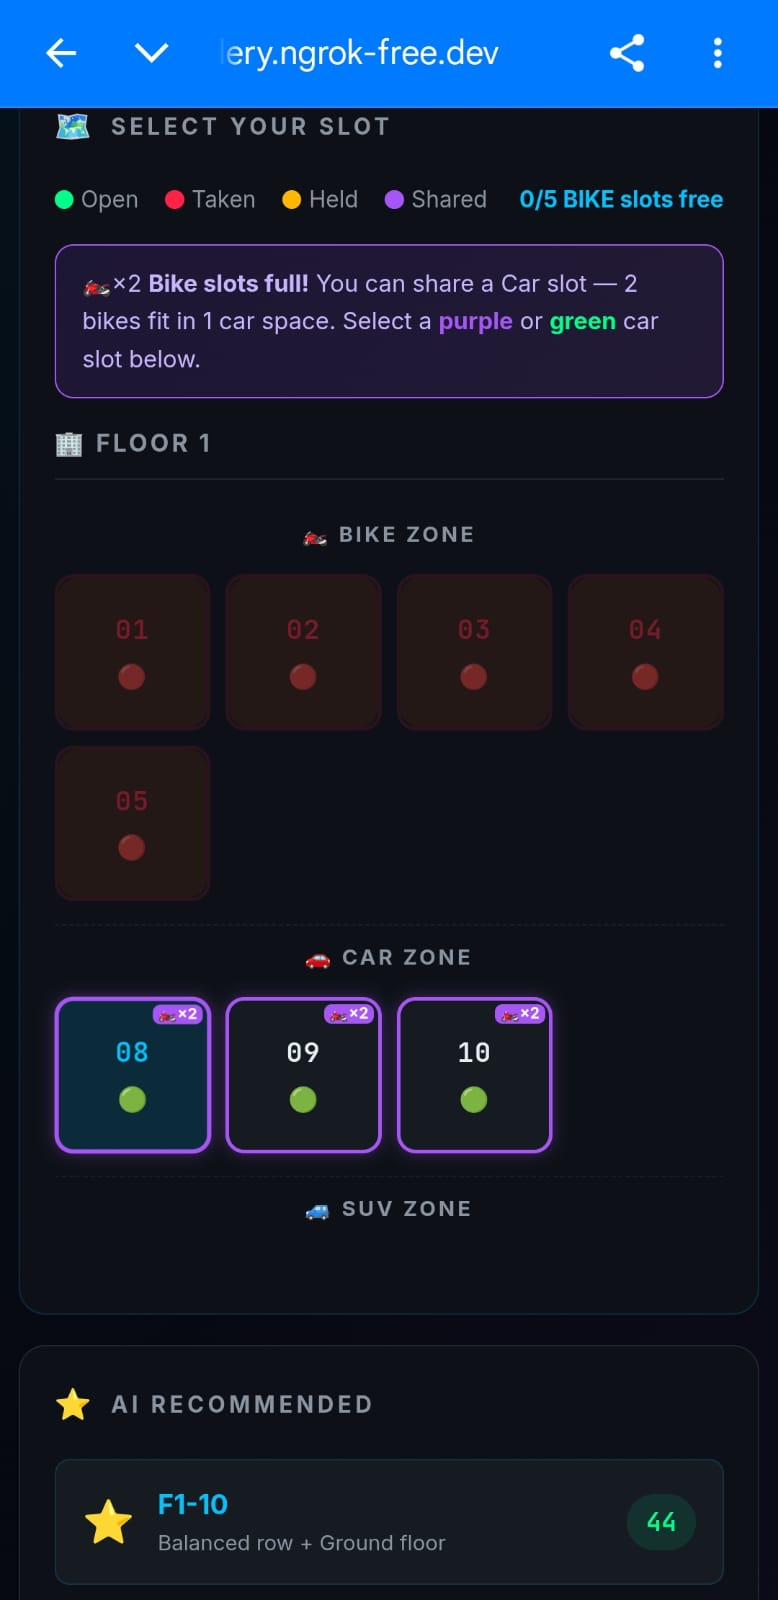
\includegraphics[width=0.85\textwidth]{../images/carsuv.jpeg}
    \caption{Car-to-SUV Overflow — Mobile UI showing orange-highlighted SUV slots available for car overflow when all Car slots are full. Cars are charged at the standard Car rate.}
    \label{fig:carsuv}
\end{figure}

As shown in Figure~\ref{fig:carsuv}, when all 5 car slots are occupied, the system dynamically highlights vacant SUV slots with orange borders and a descriptive banner. The rate displayed confirms the Car rate is applied, not the SUV rate.

% ══════════════════════════════════════════════════════════
%  SECTION 4: RESULTS
% ══════════════════════════════════════════════════════════
\section{Results and Outcomes}

\subsection{Features Delivered}

\begin{table}[H]
\centering
\caption{Feature Delivery Status}
\begin{tabular}{|l|c|l|}
\hline
\textbf{Feature} & \textbf{Status} & \textbf{Notes} \\
\hline
areCarSlotsFull() & \checkmark & Stream API filter \\
\hline
Overflow detection in API & \checkmark & Validates car slots full \\
\hline
overflowSlot JSON flag & \checkmark & Backward-compatible \\
\hline
Orange UI indicators & \checkmark & Banner, badges, glow \\
\hline
Car rate in SUV slot & \checkmark & Zero pricing code change \\
\hline
Console logging & \checkmark & [OVERFLOW CAR→SUV] tag \\
\hline
\end{tabular}
\end{table}

\subsection{Performance Metrics}

\begin{table}[H]
\centering
\caption{Enhancement Metrics}
\begin{tabular}{|l|l|}
\hline
\textbf{Metric} & \textbf{Value} \\
\hline
Additional car capacity & +5 (using empty SUV slots) \\
\hline
Pricing code changes required & 0 \\
\hline
New enum values required & 0 \\
\hline
Build status & BUILD SUCCESS (0 errors) \\
\hline
Backward compatibility & 100\% — no existing API broken \\
\hline
\end{tabular}
\end{table}

% ══════════════════════════════════════════════════════════
%  SECTION 5: CONCLUSION
% ══════════════════════════════════════════════════════════
\section{Conclusion}

The Car-to-SUV Overflow enhancement maximizes SnapPark's parking utilization by dynamically redirecting cars to vacant SUV slots during peak periods. The implementation is deliberately minimal---only one new service method, one API validation block, and frontend UI changes---demonstrating that well-architected systems (vehicle-type-based billing) naturally support new features with minimal code changes. The pricing guarantee ensures customer fairness, and the orange visual indicators provide an intuitive user experience.

% ══════════════════════════════════════════════════════════
%  SECTION 6: LEARNING OUTCOMES
% ══════════════════════════════════════════════════════════
\section{Learning Outcomes}

\begin{itemize}
    \item \textbf{Stream API Mastery:} Used functional-style \texttt{filter()} and \texttt{count()} operations for real-time slot availability analysis.
    \item \textbf{Defensive API Design:} Implemented guard clauses that reject invalid requests before processing, preventing data corruption.
    \item \textbf{Architecture Appreciation:} Learned that vehicle-type-based billing (a design decision made early) eliminated the need for any pricing code changes.
    \item \textbf{Boolean Flag Pattern:} Used a simple boolean (\texttt{isOverflowBooking}) to toggle behavior across multiple code paths without complex conditionals.
    \item \textbf{Backward-Compatible API Extension:} Added a new JSON field (\texttt{overflowSlot}) without breaking existing mobile clients.
\end{itemize}

\end{document}
